% Бүлэг 3

\chapter{Системийн зохиомж ба хөгжүүлэлт} % Зарим нэг зөвлөмж
\label{Chapter3} % Энэ бүлэг рүү ишлэл хийх бол \ref{Chapter2} командыг ашигла 

\section{Системийн архитектур}
\paragraph{} 
Зөвлөгчийн веб систем нь веб клиент, Vercel hosting, Next.js API Routes,
backend модулиуд, өгөгдлийн сан, файл хадгалалт болон гадаад
үйлчилгээнүүдээс бүрдэнэ. Энэхүү архитектур нь хэрэглэгчийн хүсэлтийг
frontend хэсгээс backend модуль руу дамжуулж, өгөгдлийг MongoDB Atlas
дээр хадгалах, файл хадгалалтыг Vercel Blob дээр зохион байгуулах,
мөн AI зөвлөмж болон и-мэйл сануулгын үйл ажиллагааг дэмжих
зориулалттай.

Дараах зурагт системийн архитектурыг харуулж байна. Энд системийн
бүрэлдэхүүн хэсгүүд болон тэдгээрийн холбоо хамаарлыг дүрсэлсэн.

\begin{figure}[H]
    \centering
    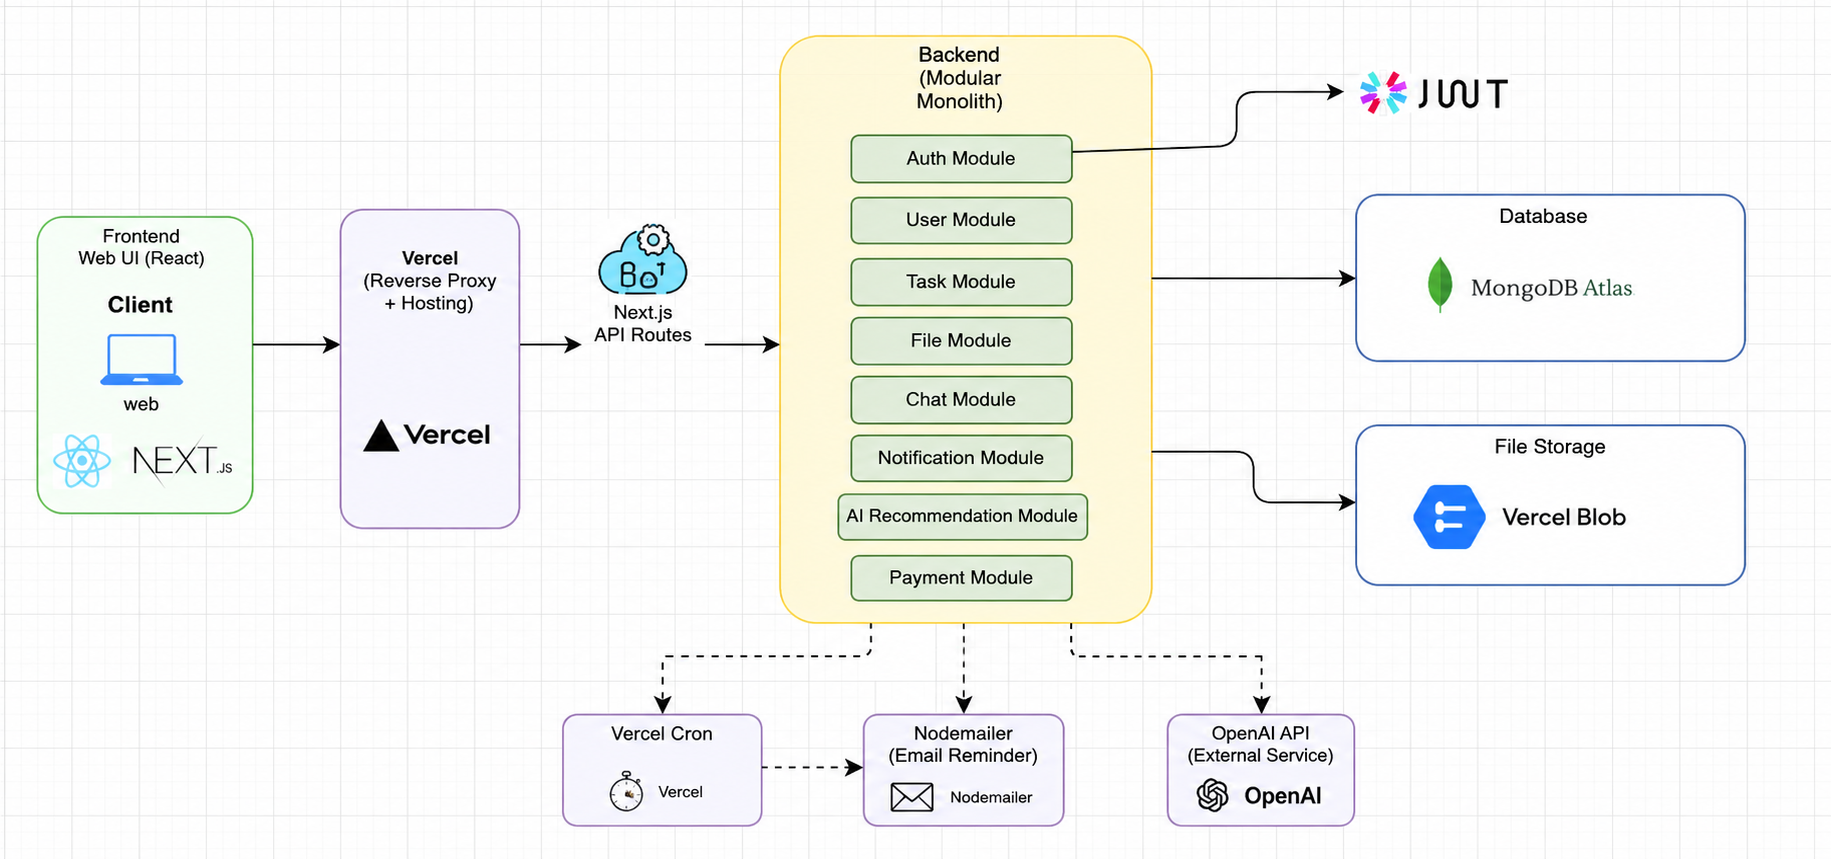
\includegraphics[scale=0.25]{Figures/chapter3/architecture.png}
    \caption{Системийн архитектур}
    \label{fig:system-architecture}
\end{figure}

\subsection*{Front-end: React болон Next.js}

Front-end хэсэг нь React болон Next.js дээр хөгжүүлэгдсэн бөгөөд
хэрэглэгчтэй харилцах үндсэн интерфейсийн үүргийг гүйцэтгэнэ.
Хэрэглэгч веб хөтчөөр дамжуулан системд хандаж, өөрийн эрхийн
дагуу системд хандана.

Front-end хэсэг нь дараах үүргүүдийг гүйцэтгэнэ. Үүнд:

\begin{itemize}
    \item Хэрэглэгчийн бүртгэл, нэвтрэлтийн интерфейс харуулах;
    \item Сурагчийн академик мэдээлэл оруулах хэсгийг харуулах;
    \item Даалгавар, файл, мэдэгдэл болон чатын интерфейсээр хангах;
    \item AI зөвлөмжийн үр дүнг хэрэглэгчид ойлгомжтой харуулах;
    \item Админ болон багшийн удирдлагын самбарыг харуулах;
    \item Backend API руу хүсэлт илгээж, буцаж ирсэн үр дүнг дэлгэцэд харуулах.
\end{itemize}

Next.js нь React дээр суурилсан framework бөгөөд web application-ийн
routing, rendering болон API Routes ашиглах боломжийг олгодог.
Ингэснээр frontend болон backend-ийн зарим үйл ажиллагааг нэг төслийн
дотор зохион байгуулах боломжтой.

\subsection*{Hosting болон Reverse Proxy: Vercel}

Систем нь Vercel платформ дээр байрших бөгөөд Vercel нь hosting болон
reverse proxy-ийн үүргийг гүйцэтгэнэ. Хэрэглэгчийн веб хөтчөөс ирсэн
хүсэлтүүд эхлээд Vercel рүү очиж, дараа нь Next.js application болон
API Routes руу дамжина.

Vercel ашигласнаар тусдаа Nginx тохируулах шаардлагагүй бөгөөд deployment,
domain холболт, HTTPS болон request routing зэрэг үйл ажиллагааг Vercel
автоматаар зохицуулна.

Vercel нь дараах үүргүүдийг гүйцэтгэнэ. Үүнд:

\begin{itemize}
    \item Веб системийг hosting хийх;
    \item Хэрэглэгчийн хүсэлтийг Next.js - рүү дамжуулах;
    \item HTTPS холболтыг дэмжих;
    \item Deployment болон production environment-ийг удирдах;
    \item Reverse proxy-ийн үүргийг гүйцэтгэх.
\end{itemize}

\subsection*{Back-end: Next.js API Routes}

Backend хэсэг нь Next.js API Routes ашиглан хөгжүүлэгдсэн бөгөөд
тусдаа Express.js сервер ашиглахгүй. API Routes нь хэрэглэгчийн
хүсэлтийг хүлээн авч, backend модулиудын бизнес логикийг ажиллуулан,
өгөгдлийн сан болон гадаад үйлчилгээнүүдтэй холбогдоно.

Backend нь дараах үүргүүдийг гүйцэтгэнэ. Үүнд:

\begin{itemize}
    \item Хэрэглэгчийн бүртгэл, нэвтрэлт болон эрхийн шалгалт хийх;
    \item Сурагч, зөвлөх багш, админ болон багшийн мэдээллийг удирдах;
    \item Даалгавар үүсгэх, оноох, төлөв шинэчлэх үйлдлийг боловсруулах;
    \item Файл байршуулах болон файлын metadata хадгалах;
    \item AI Recommendation Module-ийг ажиллуулж сургуулийн зөвлөмж гаргах;
    \item Төлбөрийн мэдээлэл болон subscription төлөвийг удирдах;
    \item Мэдэгдэл болон и-мэйл сануулга илгээх үйл ажиллагааг зохицуулах.
\end{itemize}

\subsection*{Backend архитектур: Modular Monolith}

Backend нь Modular Monolith архитектурын зарчмаар зохион байгуулагдсан.
Энэ нь системийн бүх backend логик нэг application дотор байрлах боловч
дотооддоо тусдаа модулиудад хуваагдана гэсэн үг юм. Модуль бүр өөрийн
үүрэгтэй бөгөөд кодын зохион байгуулалт, засвар үйлчилгээ болон цаашдын
өргөтгөлийг хялбар болгоно.

Backend хэсэг дараах үндсэн модулиудаас бүрдэнэ. Үүнд:

\begin{itemize}
    \item \textbf{Auth Module} -- хэрэглэгчийн бүртгэл, нэвтрэлт, JWT token болон эрхийн шалгалтыг хариуцна;
    \item \textbf{User Module} -- сурагч, зөвлөх багш, админ, багш болон супер админы мэдээллийг удирдана;
    \item \textbf{Task Module} -- даалгавар үүсгэх, оноох, төлөв шинэчлэх үйл ажиллагааг хариуцна;
    \item \textbf{File Module} -- essay, transcript, CV, recommendation зэрэг файлуудыг удирдана;
    \item \textbf{Chat Module} -- сурагч болон зөвлөх багшийн хоорондын харилцааг зохицуулна;
    \item \textbf{Notification Module} -- мэдэгдэл болон сануулгын мэдээллийг үүсгэж хэрэглэгчид хүргэнэ;
    \item \textbf{AI Recommendation Module} -- сурагчийн академик мэдээлэлд үндэслэн тохирох сургуулийн зөвлөмж боловсруулна;
    \item \textbf{Payment Module} -- сургуулийн жилийн ашиглалтын төлбөр болон subscription төлөвийг удирдана.
\end{itemize}

Modular Monolith архитектур нь microservice шиг олон тусдаа сервер шаарддаггүй
боловч кодын түвшинд модулиудыг салгаж зохион байгуулах давуу талтай.
Ингэснээр системийн хөгжүүлэлт илүү ойлгомжтой, өргөтгөхөд хялбар болно.

\subsection*{Өгөгдлийн сан: MongoDB Atlas}

Системийн үндсэн өгөгдлийг MongoDB Atlas дээр хадгална. MongoDB Atlas нь
cloud database үйлчилгээ бөгөөд хэрэглэгчийн мэдээлэл, даалгавар, файл,
чат, мэдэгдэл, төлбөр болон AI зөвлөмжийн мэдээллийг хадгалахад ашиглагдана.

Өгөгдлийн санд дараах мэдээллүүд хадгалагдана. Үүнд:

\begin{itemize}
    \item Хэрэглэгчийн үндсэн мэдээлэл;
    \item Сурагчийн академик мэдээлэл;
    \item Даалгаврын мэдээлэл болон төлөв;
    \item Чатын мессежийн мэдээлэл;
    \item Мэдэгдэл болон и-мэйл сануулгын мэдээлэл;
    \item Төлбөр болон subscription-ийн төлөв;
    \item AI зөвлөмжийн үр дүн;
    \item Байршуулсан файлын metadata болон URL.
\end{itemize}

Систем нь тусдаа UserDB гэх мэт олон өгөгдлийн сан ашиглахгүй бөгөөд
MongoDB Atlas дээр нэг database ашиглан collection-уудаар өгөгдлүүдийг
зохион байгуулна.

\subsection*{Файл хадгалалт: Vercel Blob}

Системд байршуулсан файлуудыг Vercel Blob ашиглан хадгална. Essay,
transcript, CV, recommendation letter болон зөвлөх багшийн загвар файлууд
зэрэг том хэмжээтэй файлуудыг өгөгдлийн санд шууд хадгалахгүй. Харин
Vercel Blob дээр хадгалж, MongoDB Atlas дээр тухайн файлын нэр, төрөл,
URL, огноо зэрэг metadata-г хадгална.

Vercel Blob нь дараах үүргүүдийг гүйцэтгэнэ. Үүнд:

\begin{itemize}
    \item Хэрэглэгчийн байршуулсан файлуудыг хадгалах;
    \item Файлын URL үүсгэх;
    \item Файлыг дахин татах болон харах боломж олгох;
    \item Файлын хадгалалтыг backend-ээс тусгаарлах.
\end{itemize}

\subsection*{AI Recommendation: OpenAI API}

AI Recommendation Module нь сурагчийн академик мэдээлэлд үндэслэн
тохирох их, дээд сургуулийн зөвлөмж боловсруулах үүрэгтэй. Энэхүү
модуль нь OpenAI API-тай холбогдон сурагчийн GPA, шалгалтын оноо,
сонирхож буй мэргэжил, тэтгэлгийн хэрэгцээ болон гадуурх үйл
ажиллагааны мэдээллийг боловсруулна.

AI Recommendation Module дараах байдлаар ажиллана. Үүнд:

\begin{itemize}
    \item Сурагч академик мэдээллээ системд оруулна;
    \item Back-end мэдээллийг шалгаж AI Recommendation Module руу дамжуулна;
    \item AI модуль OpenAI API руу хүсэлт илгээнэ;
    \item OpenAI API сурагчийн мэдээлэлд үндэслэн зөвлөмж боловсруулна;
    \item Үр дүнг ``Safety'', ``Match'', ``Reach'' ангиллаар буцаана;
    \item Back-end үр дүнг MongoDB Atlas дээр хадгалж, frontend рүү дамжуулна.
\end{itemize}

Ингэснээр сурагч өөрийн академик үзүүлэлтэд тохирох сургуулиудыг
ангилсан байдлаар харах боломжтой болно.

\subsection*{И-мэйл сануулга: Vercel Cron болон Nodemailer}

Даалгаврын хугацаа дөхсөн үед сурагчдад автоматаар и-мэйл сануулга
илгээхийн тулд Vercel Cron болон Nodemailer ашиглана. Vercel Cron нь
тодорхой хугацааны давтамжтайгаар backend endpoint-ийг ажиллуулж,
хугацаа дөхсөн даалгавруудыг шалгана. Nodemailer нь тухайн сурагчийн
цахим шуудан руу сануулга илгээх үүрэгтэй.

Энэ процесс дараах байдлаар ажиллана. Үүнд:

\begin{itemize}
    \item Vercel Cron тогтсон хугацаанд reminder endpoint-ийг дуудна;
    \item Back-end MongoDB Atlas-аас хугацаа дөхсөн даалгавруудыг хайна;
    \item Сануулга авах тохиргоотой сурагчдыг шүүнэ;
    \item Nodemailer ашиглан тухайн сурагчийн имэйл рүү сануулга илгээнэ;
    \item Илгээсэн сануулгын мэдээлэл notification collection-д хадгалагдана.
\end{itemize}

Энэхүү шийдэл нь сурагчдад даалгаврын хугацааг мартахгүй байх боломж
олгож, зөвлөх багшийн гараар сануулах ажлыг багасгана.

\subsection*{Төлбөрийн үйлчилгээ: JUUT}

Системийн жилийн ашиглалтын хураамж болон сургуулийн subscription
төлөвийг Payment Module удирдана. Төлбөрийн процесс нь JUUT
үйлчилгээтэй холбогдон төлбөрийн баталгаажуулалт хийх байдлаар
ажиллана.

Төлбөрийн модуль дараах үүргүүдийг гүйцэтгэнэ. Үүнд:

\begin{itemize}
    \item Сургуулийн төлбөрийн мэдээллийг үүсгэх;
    \item Төлбөрийн төлөвийг шалгах;
    \item Төлбөр амжилттай бол сургуулийн эрхийг сунгах;
    \item Төлбөр төлөгдөөгүй бол сургуулийн эрхийг түр хязгаарлах;
    \item Төлбөрийн түүхийг MongoDB Atlas дээр хадгалах.
\end{itemize}

Ингэснээр супер админ сургуулиудын төлбөр, эрх болон subscription-ийн
төлөвийг нэгдсэн байдлаар удирдах боломжтой болно.

\section{Зохиомжийн шатны класс диаграмм}
\paragraph{}
Зөвлөгчийн веб системийн зохиомжийн шатны класс диаграммд
системийн хэрэглэгчийн интерфейс, бизнес логик болон өгөгдлийн
объектуудыг \say{boundary}, \say{control}, \say{entity} гэсэн
стерео төрлүүдээр ангилан тодорхойлсон.

\say{boundary} төрлийн классууд нь хэрэглэгчтэй харилцах дэлгэцийн
хэсгийг илэрхийлнэ. Үүнд \say{LoginPage}, \say{DashboardPage},
\say{SchoolAdminPage}, \say{TaskPage}, \say{FilePage},
\say{ChatPage}, \say{RecommendationPage},
\say{RecommendationLetterPage}, \say{AdmissionResultPage},
\say{PaymentPage}, \say{NotificationPanel} зэрэг классууд багтана.

\say{control} төрлийн классууд нь хэрэглэгчийн хүсэлтийг хүлээн авч,
боловсруулан холбогдох өгөгдлийн классуудтай харилцах үүрэгтэй.
Үүнд \say{AuthAPIRoute}, \say{UsersAPIRoute}, \say{SchoolsAPIRoute},
\say{TasksAPIRoute}, \say{FilesAPIRoute},
\say{ConversationsAPIRoute}, \say{MessagesAPIRoute},
\say{AIRecommendationAPIRoute}, \say{RecommendationLettersAPIRoute},
\say{AdmissionResultsAPIRoute}, \say{NotificationsAPIRoute},
\say{PaymentsAPIRoute} зэрэг классууд орно.

\say{entity} төрлийн классууд нь өгөгдлийн санд хадгалагдах үндсэн
объектуудыг илэрхийлнэ. Үүнд \say{User}, \say{School}, \say{Student},
\say{Counselor}, \say{SchoolAdmin}, \say{SuperAdmin},
\say{RecommendationTeacher}, \say{AcademicInfo},
\say{AIRecommendation}, \say{Task}, \say{File},
\say{Conversation}, \say{Message}, \say{Notification},
\say{RecommendationRequest}, \say{RecommendationLetter},
\say{AdmissionResult}, \say{Payment} зэрэг классууд багтана.

Зураг \ref{fig:z-class}-д эдгээр классуудын аттрибут, функц болон
хоорондын холбоо хамаарлыг харуулсан. Boundary классууд нь control
классуудтай холбогдон хэрэглэгчийн үйлдлийг дамжуулж, control
классууд нь entity классуудтай холбогдон өгөгдөл боловсруулах,
хадгалах, шинэчлэх үйл ажиллагааг гүйцэтгэнэ. Ингэснээр системийн
зохиомжийн түвшинд хэрэглэгчийн интерфейс, backend API route болон
өгөгдлийн объектуудын уялдаа холбоо тодорхой харагдана.
\begin{figure}[H]
    \centering
    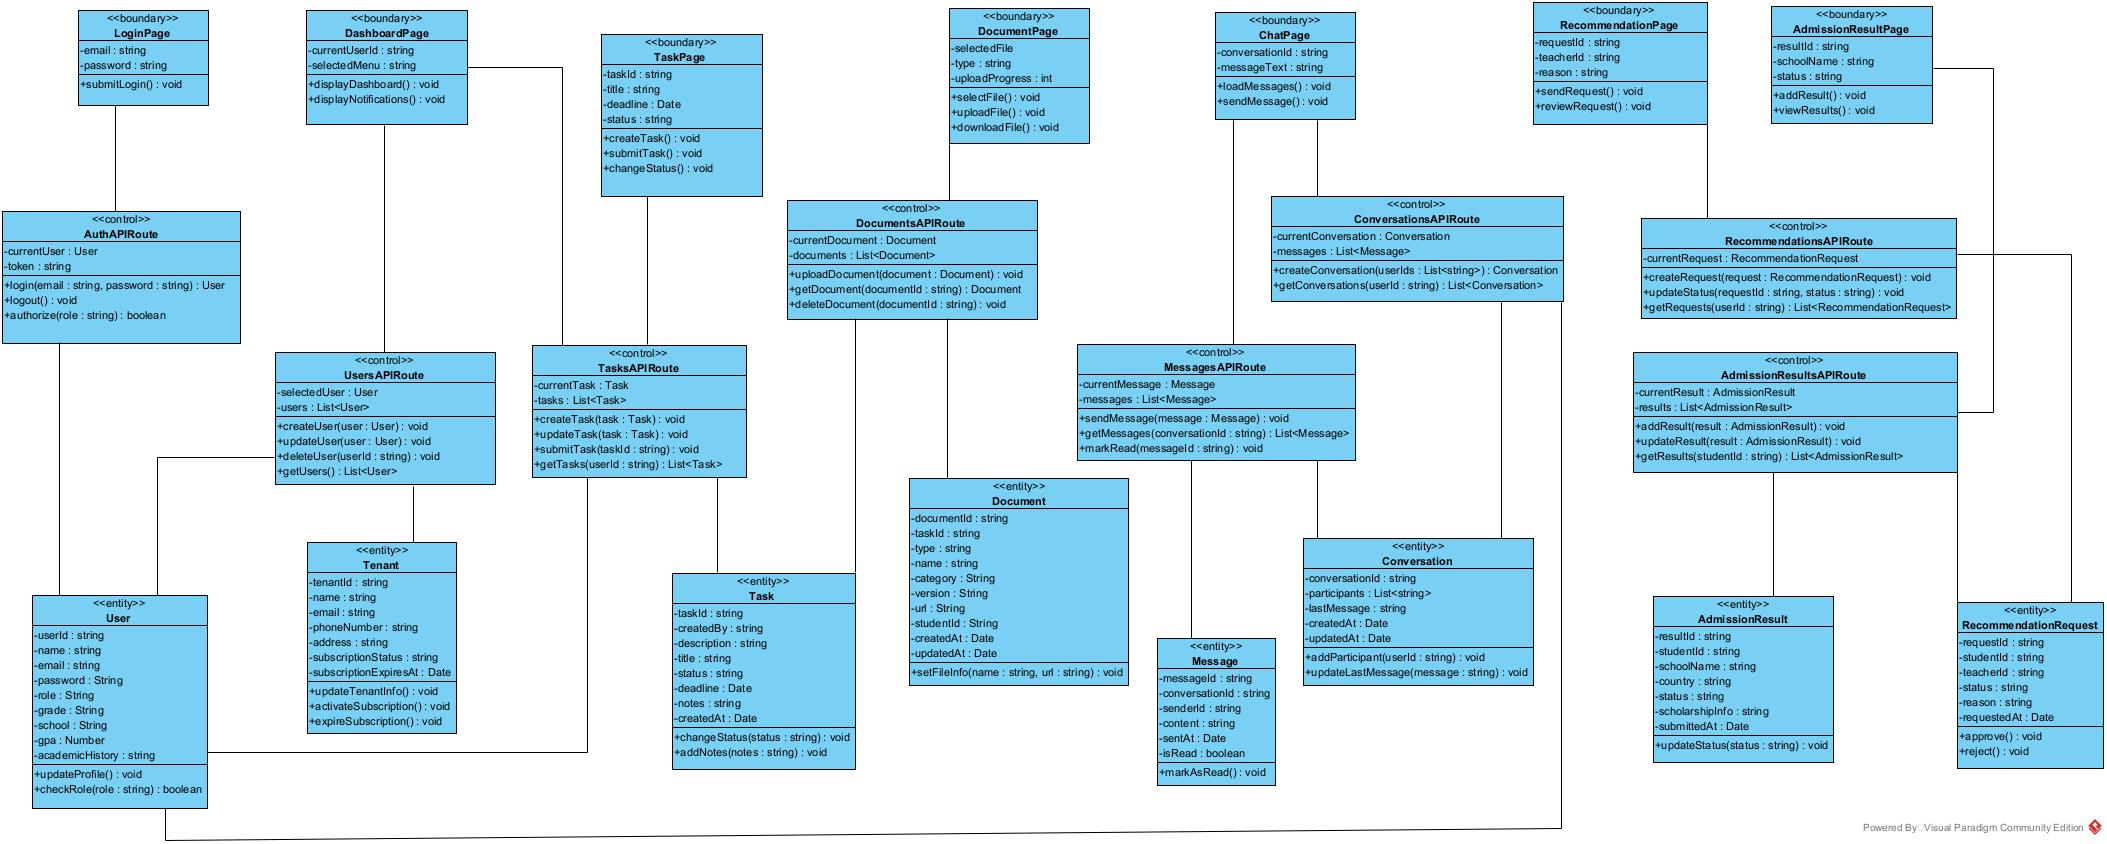
\includegraphics[height=0.4\textheight, keepaspectratio, angle=90]{Figures/chapter3/зохиомжийн класс диаграмм.jpg}
    \caption{Класс диаграмм}
    \label{fig:z-class}
\end{figure}

\section{Зохиомжийн дарааллын диаграмм}

\paragraph{}
Дарааллын диаграмм нь системийн объектуудын хоорондын харилцааг
цаг хугацааны дарааллаар дүрслэх зориулалттай UML диаграммын нэг
төрөл юм. Энд хэрэглэгч болон системийн бүрэлдэхүүн хэсгүүдийн
хоорондох мессежийн урсгалыг тодорхойлсон.

Системийн гол юзкейсүүд болох нэвтрэх, даалгавар үүсгэх болон
тодорхойлох захидлын хүсэлт илгээх үйл ажиллагааг дарааллын
диаграммаар дүрсэлсэн.


\subsection*{Даалгавар үүсгэх дарааллын диаграмм}

\par \noindent Зураг \ref{fig:seq-task}-д зөвлөх багш сурагчид даалгавар
үүсгэх үйл ажиллагааны дарааллыг харуулсан. Зөвлөх багш TaskPage-ээс
даалгаврын мэдээллийг оруулан хадгалахад TasksAPIRoute хүсэлтийг
хүлээн авна. JWT token-ийн тусламжтайгаар хэрэглэгчийн эрхийг
баталгаажуулсны дараа даалгаврын мэдээллийг MongoDB Atlas-д хадгалж,
сурагчид NotificationsAPIRoute дамжуулан мэдэгдэл илгээнэ.

\begin{figure}[H]
    \centering
    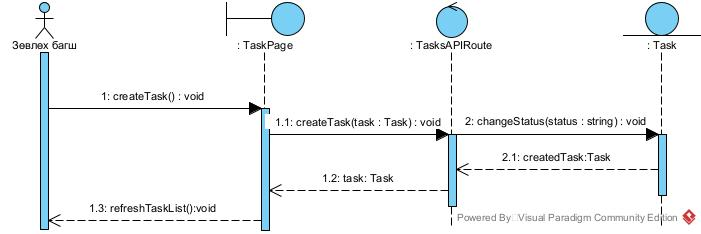
\includegraphics[width=0.85\textwidth]{Figures/chapter3/Даалгавар үүсгэх дарааллын диаграм.jpg}
    \caption{Даалгавар үүсгэх дарааллын диаграмм}
    \label{fig:seq-task}
\end{figure}

\subsection*{Тодорхойлох захидлын хүсэлт илгээх дарааллын диаграмм}

\par \noindent Зураг \ref{fig:seq-rec}-д сурагч тодорхойлох захидал
бичих багшид хүсэлт илгээх үйл ажиллагааны дарааллыг харуулсан.
Сурагч RecommendationLetterPage-ээс захидлын хүсэлт үүсгэхэд
RecommendationLettersAPIRoute хүсэлтийг хүлээн авч, MongoDB Atlas-д
хадгалана. Дараа нь холбогдох багшид NotificationsAPIRoute-аар дамжуулан
шинэ хүсэлт ирсэн тухай мэдэгдэл автоматаар илгээгдэнэ.

\begin{figure}[H]
    \centering
    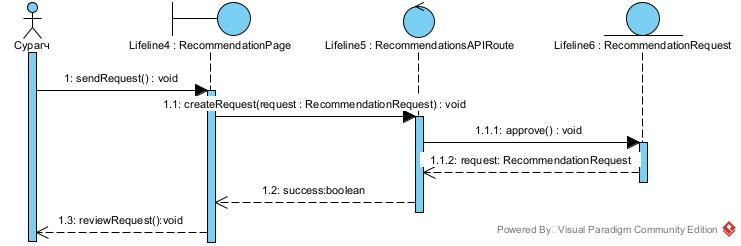
\includegraphics[width=0.85\textwidth]{Figures/chapter3/Тодорхойлох захидал бичүүлэх хүсэлт илгээх дарааллын диаграмм.jpg}
    \caption{Тодорхойлох захидлын хүсэлт илгээх дарааллын диаграмм}
    \label{fig:seq-rec}
\end{figure}

% \clearpage
\section{Хөгжүүлсэн системийн интерфейс}

\paragraph{} Энэ хэсэгт хөгжүүлэгдсэн сургуулийн зөвлөгчийн веб системийн үндсэн хуудаснуудын интерфейсийг тайлбарлана. Систем нь сурагч болон зөвлөх багшид зориулсан тусдаа dashboard-тай бөгөөд хэрэглэгч бүр өөрийн эрхийн дагуу харгалзах интерфейст нэвтэрнэ.

\par \noindent Зураг \ref{fig:studentHome}-д сурагчийн нүүр хуудасны интерфейсийг харуулсан. Энэхүү хуудаст сурагч өөрт оноогдсон даалгаврын ерөнхий мэдээлэл, гүйцэтгэлийн явц болон элсэлтийн процессийн төлөвийг нэг дороос харах боломжтой. Dashboard нь сурагчийн даалгавар, файл болон мэдэгдлийн товч тоймыг харуулна.

\begin{figure}[H]
    \centering
    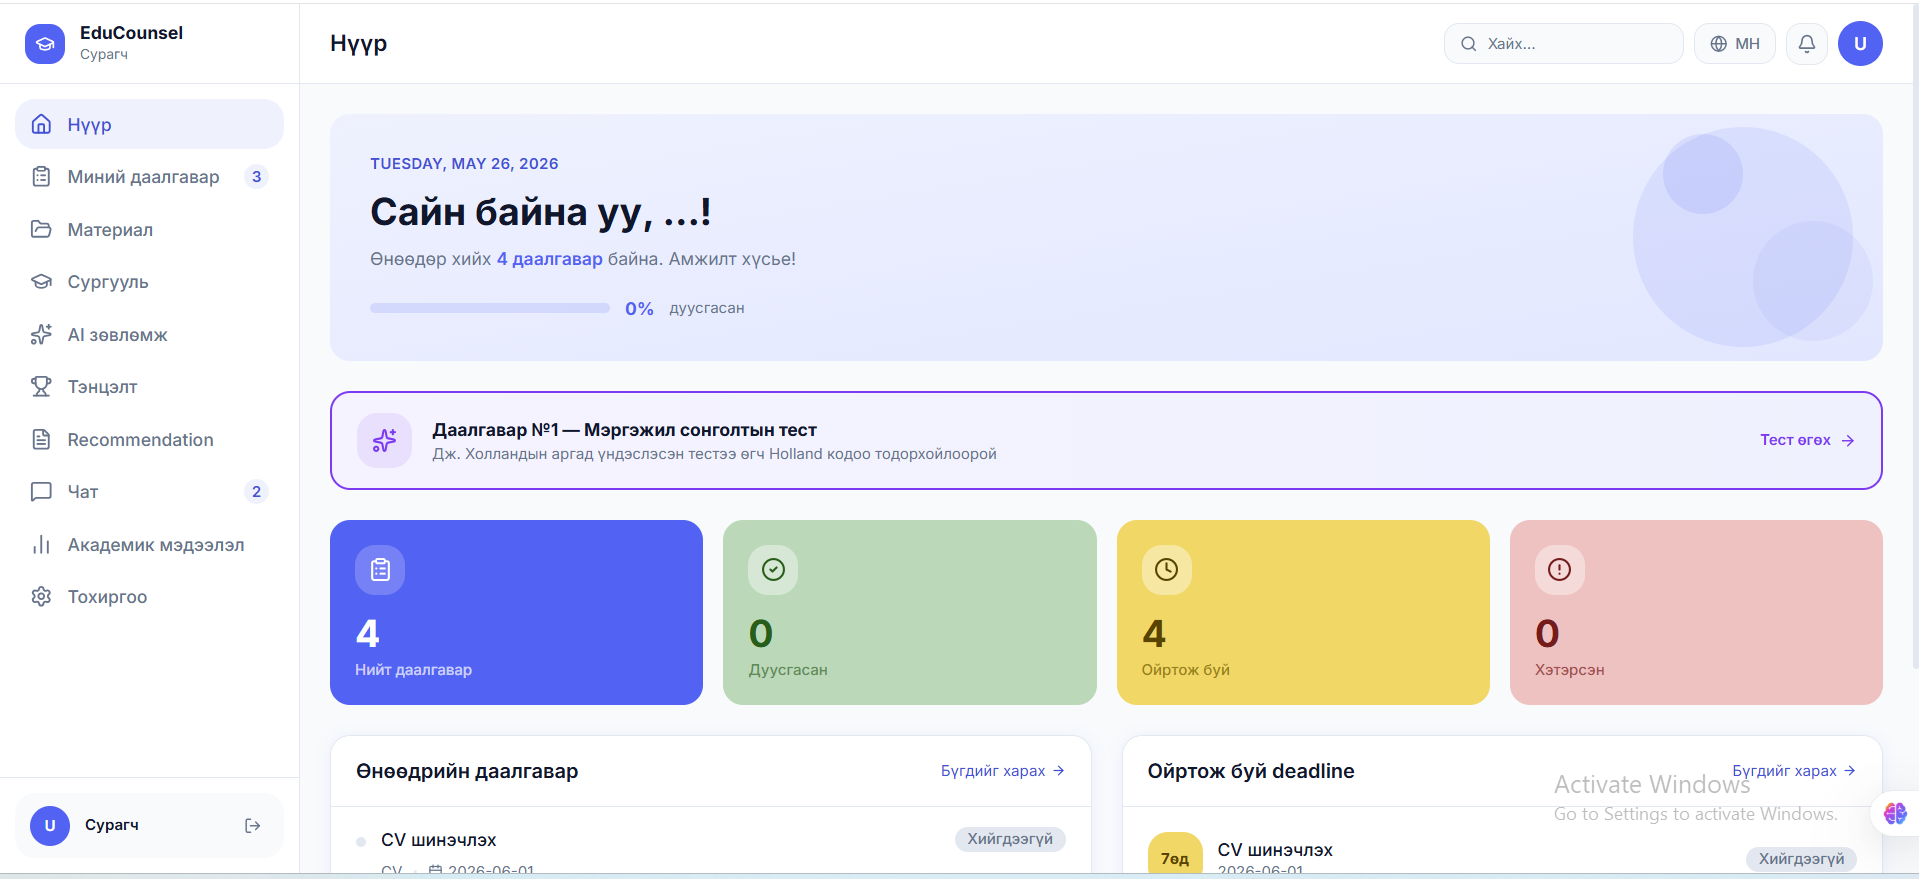
\includegraphics[width=0.6\textwidth]{Figures/chapter3/studentHome.png}
    \caption{Сурагчийн нүүр хуудасны интерфейс}
    \label{fig:studentHome}
\end{figure}

\par \noindent Зураг \ref{fig:counselorHome}-д зөвлөх багшийн нүүр хуудасны интерфейсийг харуулсан. Зөвлөх багш нь энэхүү хуудаснаас өөрийн хариуцсан сурагчдын тоо, нийт даалгаврын явц болон ирсэн мэдэгдлийн мэдээллийг харна. Dashboard нь зөвлөх багшид сурагч бүрийн ерөнхий байдлыг хурдан дүгнэх боломж олгодог.

\begin{figure}[H]
    \centering
    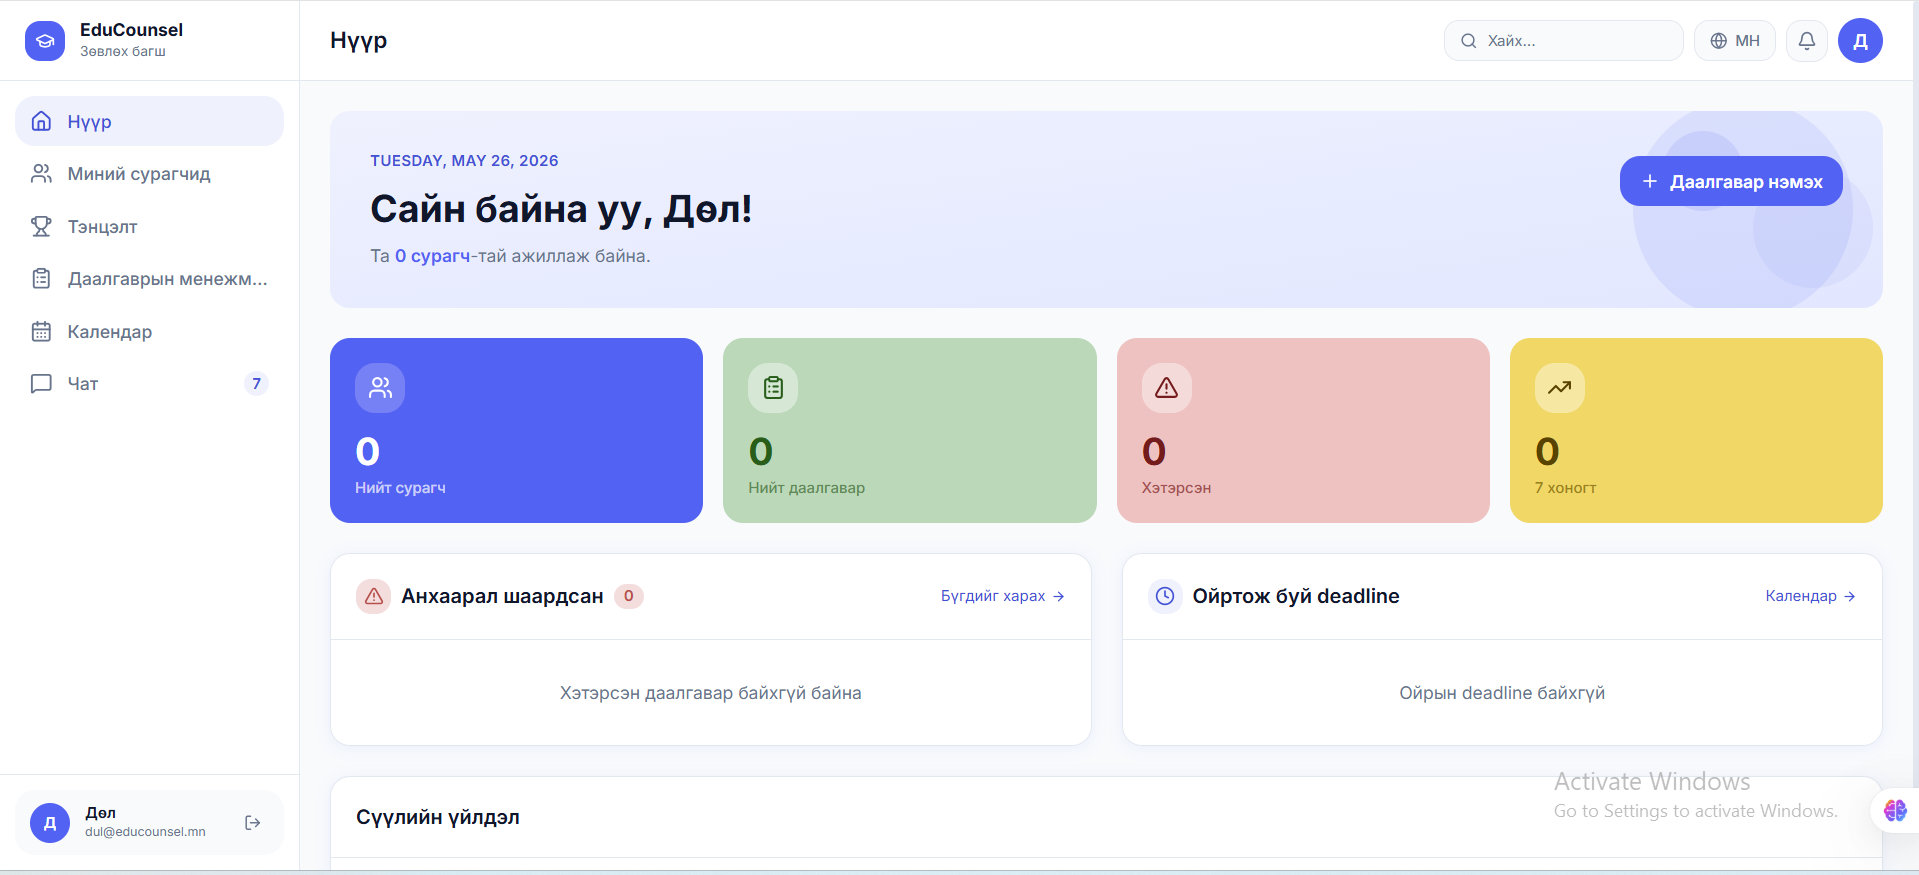
\includegraphics[width=0.6\textwidth]{Figures/chapter3/counselorHome.png}
    \caption{Зөвлөх багшийн нүүр хуудасны интерфейс}
    \label{fig:counselorHome}
\end{figure}

\par \noindent Зураг \ref{fig:counselorMyStudent}-д зөвлөх багшийн ``Миний сурагчид'' хуудасны интерфейсийг харуулсан. Энэ хуудаст зөвлөх багш өөрийн хариуцсан сурагчдын жагсаалтыг харж, сурагч бүрийн элсэлтийн явц, гүйцэтгэсэн даалгаврын тоо болон холбогдох мэдээллийг нэг дороос хянах боломжтой.

\begin{figure}[H]
    \centering
    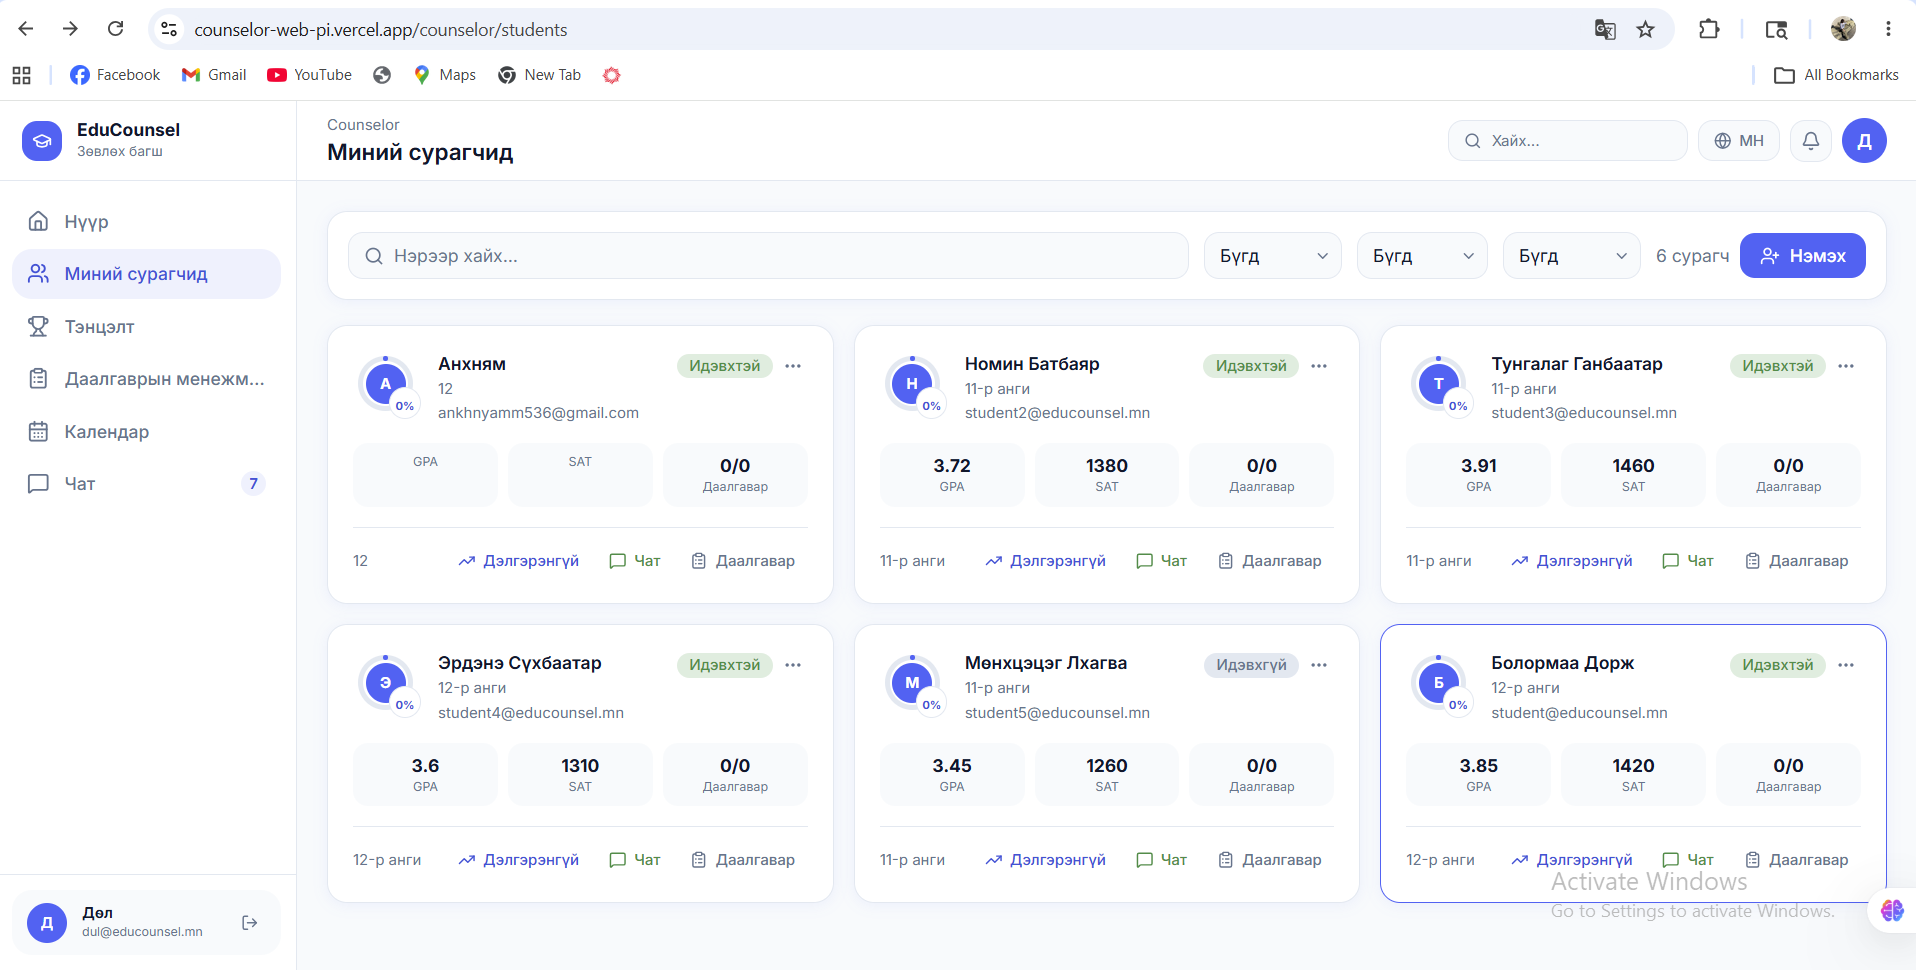
\includegraphics[width=0.6\textwidth]{Figures/chapter3/counselorMyStudent.png}
    \caption{Зөвлөх багшийн сурагчдын жагсаалтын интерфейс}
    \label{fig:counselorMyStudent}
\end{figure}

\par \noindent Зураг \ref{fig:counselorTentselt}-д зөвлөх багшийн элсэлтийн дүнгийн хуудасны интерфейсийг харуулсан. Энэ хуудаст сурагчдын тэнцсэн болон татгалзсан сургуулиудын мэдээлэл, тэтгэлгийн хэмжээ болон элсэлтийн ерөнхий статистикийг харуулна. Зөвлөх багш сурагч бүрийн элсэлтийн үр дүнг тайлан хэлбэрээр хянаж болно.

\begin{figure}[H]
    \centering
    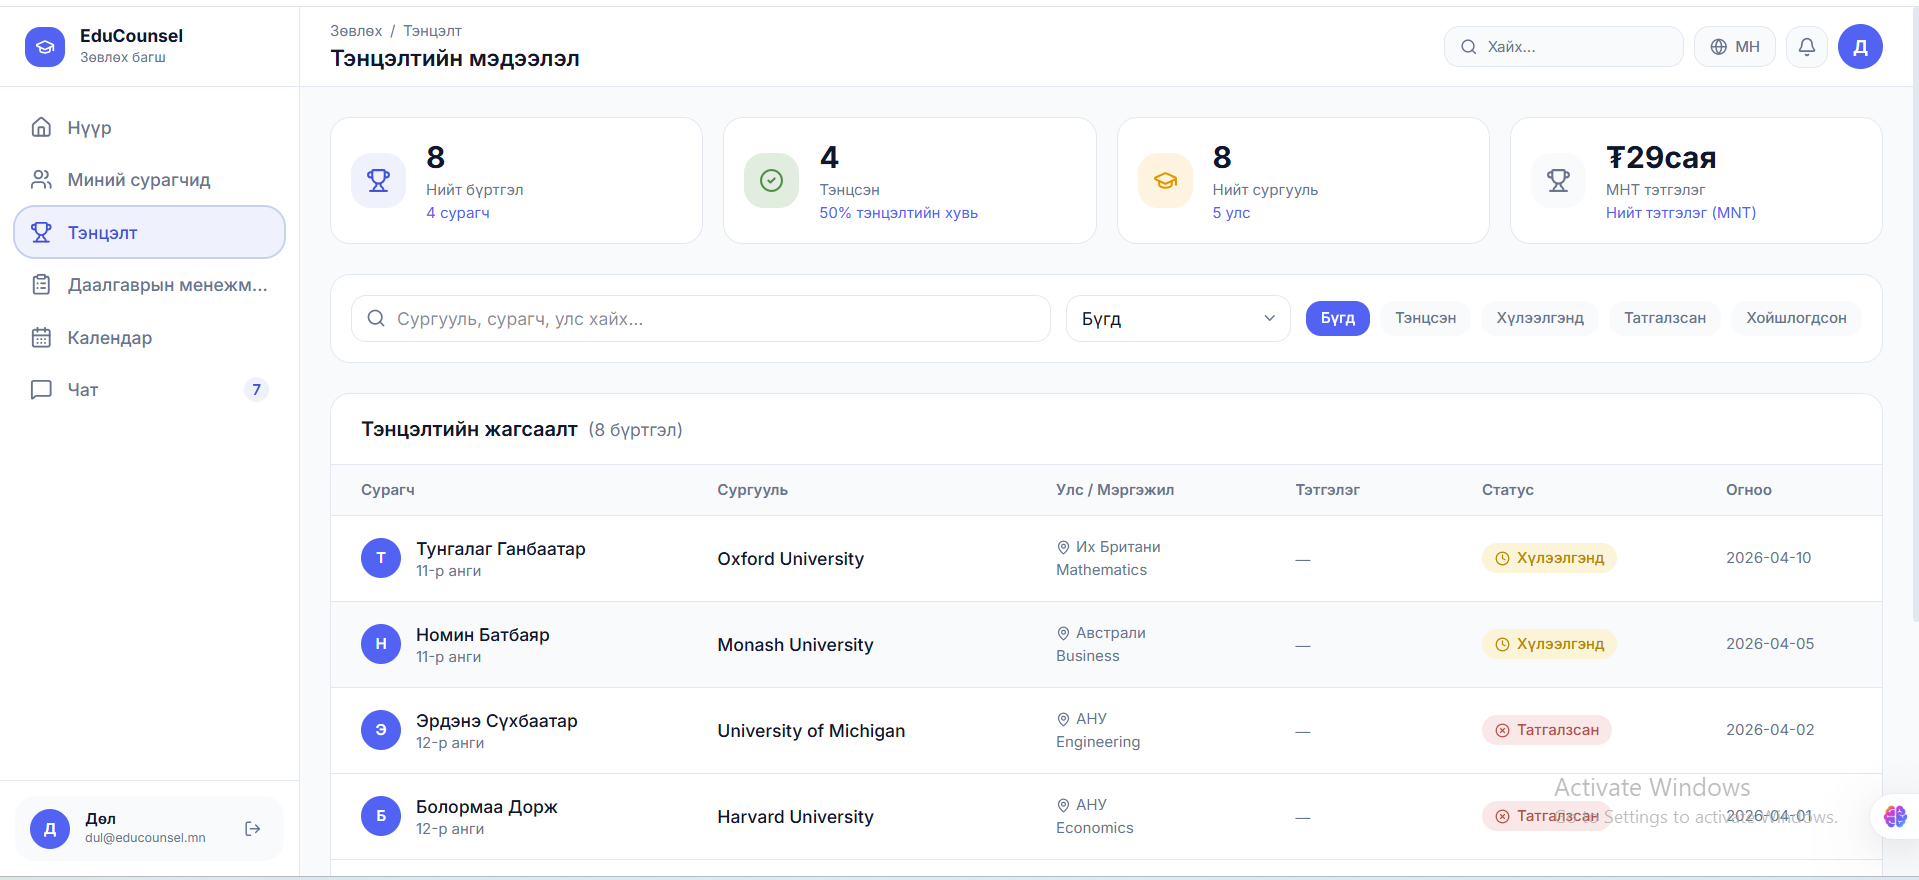
\includegraphics[width=0.6\textwidth]{Figures/chapter3/counselorTentselt.png}
    \caption{Зөвлөх багшийн элсэлтийн дүнгийн интерфейс}
    \label{fig:counselorTentselt}
\end{figure}

\section{Системд хийгдсэн тест}

\paragraph{}
Хөгжүүлэгдсэн системийн чанар, найдвартай байдал болон хэрэглэгчийн
туршлагыг баталгаажуулах зорилгоор альфа болон бета тестийг тус тус
хийж гүйцэтгэсэн.

\subsection*{Альфа тест}

Альфа тестийг хөгжүүлэлтийн явцад системийн дотоод баг хийж гүйцэтгэв.
Тестийн зорилго нь системийн үндсэн функциональ шаардлагуудыг биелүүлж
байгаа эсэхийг шалгах, алдааг эрт илрүүлж засах явдал байв.

Альфа тестийн хүрээнд дараах чиглэлүүдийг шалгасан. Үүнд:

\begin{itemize}
    \item \textbf{Баталгаажуулалтын тест:} Хэрэглэгчийн бүртгэл,
    нэвтрэлт, нууц үг сэргээх болон JWT token-ийн хүчинтэй хугацааг
    шалгасан. Буруу нэвтрэлтийн оролдлогод зөв алдааны мэдэгдэл
    гарч байгааг баталгаажуулсан.

    \item \textbf{Даалгаврын модулийн тест:} Зөвлөх багш даалгавар
    үүсгэх, засах, устгах болон сурагчид оноох үйлдлүүд зөв ажиллаж
    байгааг, сурагч даалгаврын төлөвийг шинэчлэх боломжтойг шалгасан.

    \item \textbf{Файлын модулийн тест:} Файл байршуулах, татаж авах,
    өмнөх хувилбаруудыг харах болон зөвхөн зөвшөөрөгдсөн форматын
    файлыг хүлээн авч байгааг шалгасан.

    \item \textbf{AI зөвлөмжийн тест:} Сурагчийн академик мэдээлэлд
    үндэслэн "Safety", "Match", "Reach" ангилалтай зөвлөмж зөв
    гарч байгааг шалгасан.

    \item \textbf{Чат болон мэдэгдлийн тест:} Сурагч болон зөвлөх
    багшийн хоорондын мессеж солилцол, мэдэгдэл цаг тухайд нь
    ирж байгааг шалгасан.

    \item \textbf{Хандалтын эрхийн тест:} Хэрэглэгч бүр зөвхөн өөрийн
    эрхийн хүрээнд хандах боломжтой эсэхийг Role-Based Access Control
    зарчмаар шалгасан.
\end{itemize}

Альфа тестийн явцад илэрсэн алдааг засаж, системийн үндсэн
үйл ажиллагааг тогтворжуулсны дараа бета тест руу шилжсэн.

\subsection*{Бета тест}

Бета тестийг бодит хэрэглэгчдийн оролцоотойгоор хийж гүйцэтгэсэн.
Системийг туршсан хэрэглэгчдэд зөвлөх багш болон сурагчид хамрагдав.
Тестийн зорилго нь системийн ашиглахад хялбар байдал, гүйцэтгэл болон
хэрэглэгчийн туршлагыг бодит нөхцөлд үнэлэх явдал байв.

Бета тестийн явцад хэрэглэгчдэд дараах даалгавруудыг гүйцэтгүүлсэн. Үүнд:

\begin{itemize}
    \item Системд бүртгүүлж нэвтрэх;
    \item Академик мэдээлэл оруулж AI зөвлөмж авах;
    \item Даалгавраа харж, гүйцэтгэлийн түвшинг шинэчлэх;
    \item Файл байршуулж, зөвлөх багштайгаа чатлах;
    \item Тодорхойлох захидлын хүсэлт илгээх.
\end{itemize}

Туршилтын дараа хэрэглэгчдээс санал хүсэлт цуглуулж, системийн
интерфейс болон үйл ажиллагааны талаарх үнэлгээг тэмдэглэв.
Бета тестийн үр дүнд системийн хариу хурд хангалттай, интерфейс
ойлгомжтой болох нь нотлогдсон.

\subsection*{Тестийн тохиолдлууд}

Системийн үндсэн функцүүдийг шалгахдаа хэрэглэгчийн бодит ажлын урсгалд
тулгуурласан тестийн тохиолдлуудыг боловсруулсан. Доорх хүснэгтэд гол
үйлдлүүдийн хүлээгдэж буй үр дүн, бодит үр дүн болон тестийн төлөвийг
нэгтгэн харуулав.

\begin{table}[H]
\centering
\caption{Системийн үндсэн функцүүдийн тестийн тохиолдлууд}
\label{tab:system-test-cases}
{\small
\renewcommand{\arraystretch}{1.25}
\begin{tabular}{|p{3.2cm}|p{4.2cm}|p{4.2cm}|p{2cm}|}
\hline
\textbf{Тестийн тохиолдол} & \textbf{Хүлээгдэж буй үр дүн} & \textbf{Бодит үр дүн} & \textbf{Төлөв} \\
\hline
Нэвтрэх & Зөв и-мэйл, нууц үг оруулахад хэрэглэгч өөрийн эрхийн дагуу системд нэвтэрнэ. & Хэрэглэгч амжилттай нэвтэрч, тухайн үүрэгт тохирох нүүр хуудас руу шилжсэн. & Амжилттай \\
\hline
Даалгавар үүсгэх & Зөвлөх багш сурагчид даалгавар үүсгэж онооно. & Даалгавар үүсэж, сурагчийн даалгаврын жагсаалтад харагдсан. & Амжилттай \\
\hline
Даалгаврын явц шинэчлэх & Сурагч даалгаврын гүйцэтгэлийн түвшин болон төлөвийг шинэчилнэ. & Шинэчилсэн төлөв хадгалагдаж, зөвлөх багшийн интерфейст туссан. & Амжилттай \\
\hline
Баримт бичиг байршуулах & Зөвшөөрөгдсөн форматтай файл системд байршуулж, metadata хадгалагдана. & Файл байршуулж, татаж авах холбоос болон мэдээлэл хадгалагдсан. & Амжилттай \\
\hline
Тодорхойлох захидлын хүсэлт илгээх & Сурагч багшид тодорхойлох захидлын хүсэлт илгээнэ. & Хүсэлт үүсэж, багшийн хүсэлтийн жагсаалтад харагдсан. & Амжилттай \\
\hline
Тодорхойлох захидал илгээх & Багш бичсэн захидлаа системээр дамжуулан илгээнэ. & Захидлын файл хадгалагдаж, сурагч болон зөвлөх багшид харагдсан. & Амжилттай \\
\hline
Элсэлтийн үр дүн бүртгэх & Сурагч эсвэл зөвлөх багш элсэлтийн үр дүнг бүртгэнэ. & Элсэлтийн төлөв болон тэтгэлгийн мэдээлэл хадгалагдсан. & Амжилттай \\
\hline
AI зөвлөмж үүсгэх & Академик мэдээлэлд үндэслэн ``Safety'', ``Match'', ``Reach'' ангилалтай сургуулийн зөвлөмж гарна. & AI зөвлөмж үүсэж, ангилсан байдлаар интерфейст харагдсан. & Амжилттай \\
\hline
Мэдэгдэл болон и-мэйл сануулга илгээх & Даалгаврын хугацаа дөхөхөд систем мэдэгдэл болон и-мэйл сануулга илгээнэ. & Сануулгын мэдээлэл үүсэж, хэрэглэгчид мэдэгдэл хүрсэн. & Амжилттай \\
\hline
\end{tabular}
}
\end{table}

\section{Системийн нэвтрүүлэлт}

\paragraph{}
Хөгжүүлэгдсэн сургуулийн зөвлөгчийн веб систем нь Vercel платформ
дээр байрлуулагдсан. Vercel нь Next.js-ийг анх боловсруулсан компани
бөгөөд тус framework-д зориулсан хамгийн тохиромжтой байршуулалтын
платформ юм.

\subsection*{Vercel дээр байршуулах}

Системийг Vercel дээр байршуулахдаа дараах алхмуудыг дагасан.

\begin{enumerate}
    \item \textbf{GitHub репозитортой холбох:} Системийн эх кодыг
    GitHub репозиторт байрлуулж, Vercel-тэй шууд холбосон. Ингэснээр
    \texttt{main} салааны кодын өөрчлөлт бүрт Vercel автоматаар
    шинэ байршуулалт хийдэг CI/CD дамжлага тохируулагдсан.

    \item \textbf{Орчны хувьсагч тохируулах:} Системийн ажиллагаанд
    шаардлагатай нууц тохиргоонуудыг Vercel-ийн орчны хувьсагчаар
    тохируулсан. Үүнд:
    \begin{itemize}
        \item \texttt{MONGODB\_URI} --- MongoDB Atlas-ийн холболтын хаяг;
        \item \texttt{JWT\_SECRET} --- JWT token үүсгэх нууц түлхүүр;
        \item \texttt{OPENAI\_API\_KEY} --- OpenAI API-н нэвтрэх түлхүүр;
        \item \texttt{BLOB\_READ\_WRITE\_TOKEN} --- Vercel Blob-ийн хандалтын токен;
        \item \texttt{EMAIL\_USER}, \texttt{EMAIL\_PASS} --- Nodemailer-ийн и-мэйл тохиргоо.
    \end{itemize}

    \item \textbf{MongoDB Atlas тохируулах:} Өгөгдлийн санг MongoDB
    Atlas-ийн AWS Seoul бүсэд байрлуулсан. Vercel serverless
    функцийн IP хаягуудыг MongoDB Atlas-ийн хандалтын жагсаалтад
    нэмж, аюулгүй холболтыг хангасан.

    \item \textbf{Vercel Cron тохируулах:} Даалгаврын хугацааны
    сануулга илгээх Cron ажлыг \texttt{vercel.json} файлд тохируулсан.
    Өдөр бүр 08:00 цагт ажиллахаар тохируулж, зөвхөн нууц токен
    дамжуулан дуудах боломжтой хамгаалалт нэмсэн.

    \item \textbf{Домайн тохируулах:} Vercel-ийн өгч буй домайн нэрээр
    системд хандах боломжтой болгосон. HTTPS холболтыг Vercel
    автоматаар удирдана.
\end{enumerate}

\subsection*{Байршуулалтын давуу тал}

Vercel дээр байршуулсан нь дараах давуу талуудыг бий болгосон. Үүнд:

\begin{itemize}
    \item \textbf{Автомат CI/CD:} GitHub-д кодын өөрчлөлт оруулахад
    Vercel автоматаар шинэ хувилбарыг байршуулдаг тул хөгжүүлэлт
    болон нэвтрүүлэлтийн дамжлага хурдасч, алдаа гарах эрсдэл
    буурсан.

    \item \textbf{Serverless функц:} Next.js API Routes нь Vercel-д
    serverless функц хэлбэрээр ажиллах тул сервер тусад нь
    удирдах шаардлагагүй. Хэрэглэгчийн ачааллын дагуу автоматаар
    өргөтгөгдөнө.

    \item \textbf{Edge Network:} Vercel-ийн глобал edge network ашиглан
    статик хуудсуудыг хэрэглэгчийн байршилд ойр серверээс хурдан
    хүргэх боломжтой.

    \item \textbf{Preview Deployment:} Гол салбараас тусдаа
    feature branch байршуулахад Vercel тусдаа preview URL үүсгэдэг
    тул шинэ боломжуудыг туршин шалгахад хялбар болсон.
\end{itemize}

\subsection*{Цаашдын хөгжүүлэлт}

\par Системийн үндсэн хувилбар нь элсэлтийн зөвлөгөөний гол үйл ажиллагааг
цахим хэлбэрт шилжүүлэх боломжийг бүрдүүлсэн боловч хэрэглэгчийн хүрээ
тэлэхийн хэрээр дараах чиглэлүүдээр өргөтгөн хөгжүүлэх шаардлагатай.

\begin{itemize}
    \item \textbf{Мобайл аппликейшн:} Сурагч болон зөвлөх багш гар утаснаас
    даалгавар, мэдэгдэл, чат болон материалын төлөвийг шуурхай хянах
    боломжийг нэмэгдүүлэх;

    \item \textbf{WebSocket-д суурилсан бодит цагийн чат:} Одоогийн polling
    архитектурыг цаашид WebSocket шийдлээр сайжруулж, мессеж болон
    мэдэгдлийн хоцролтыг бууруулах;

    \item \textbf{Тэтгэлгийн зөвлөмж:} Сурагчийн академик үзүүлэлт,
    сонирхол болон санхүүгийн хэрэгцээнд үндэслэн тохирох тэтгэлгийн
    боломжуудыг санал болгох;

    \item \textbf{Эцэг эхийн портал:} Эцэг эхчүүд сурагчийн ерөнхий явц,
    хугацаа болон зөвлөх багшийн мэдэгдлийг харах боломжтой тусдаа
    хандалтын түвшин бий болгох;

    \item \textbf{Их сургуулийн API интеграц:} Цаашид их сургуулиудын
    admission болон scholarship мэдээллийг API-аар холбож, мэдээллийн
    шинэчлэлтийг автоматжуулах;

\end{itemize}


\section{Бүлгийн дүгнэлт}
\paragraph{} Энэ бүлэгт ерөнхийдөө системийн зохиомжийг гаргасан. Системийн архитектур, класс диаграмм, дарааллын диаграмм, өгөгдлийн ерөнхий схем, системийн прототип загвар болон хөгжүүлэгдсэн системийн интерфейсийг багтаасан. Системийн архитектурыг front-end болон back-end гэсэн үндсэн 2 хэсэгт хувааж, тэдгээр хэсгүүд дээр хийгдэх үйл ажиллагаануудыг бүдүүвч байдлаар дүрсэлсэн. Ингэхдээ front-end хэсгийг хэрэглэгчид харагдаж, хэрэглэгчтэй харилцах хэсэг, back-end хэсгийг системийн логик үйл ажиллагааг хангах хэсэг гэж тодорхойлоод REST API ашиглан тэдгээрийн дунд холболт үүсгэхээр дүрсэлсэн. Класс диаграмм дээр шинжилгээний шатны control төрлийн 6-н класс дээр нэмээд boundary төрлийн 5-н класс, entity төрлийн 2 классыг гаргаж тэдгээрийн харьцаа хамаарлыг тодорхойлсон. Шинээр тодорхойлсон классуудыг оролцуулан илүү дэлгэрэнгүй, ойлгомжтой дарааллын диаграммуудыг системийн юзкейс болгон дээр үүсгэсэн. Өгөгдлийн ерөнхий схемийг зохиомжлохдоо Хэрэглэгч, Хэрэглэгчийн файл гэсэн 2 хүснэгтүүдийг үүсгэн аттрибутуудыг тодорхойлоод, тэдгээрийг (1 : олон) харьцаагаар тодорхойлсон. Хөгжүүлэлт эхлэхээс өмнөх системийн прототип загварыг boundary төрлийн классуудын хувьд гаргасан. Мөн хөгжүүлэлтийн дараах системийн интерфейсийг хөгжүүлэгдсэн вебийн хуудас бүрээр оруулсан. 
